\PassOptionsToPackage{unicode=true}{hyperref} % options for packages loaded elsewhere
\PassOptionsToPackage{hyphens}{url}
\PassOptionsToPackage{dvipsnames,svgnames*,x11names*}{xcolor}
%
\documentclass[12pt,]{krantz}
\usepackage{lmodern}
\usepackage{amssymb,amsmath}
\usepackage{ifxetex,ifluatex}
\usepackage{fixltx2e} % provides \textsubscript
\ifnum 0\ifxetex 1\fi\ifluatex 1\fi=0 % if pdftex
  \usepackage[T1]{fontenc}
  \usepackage[utf8]{inputenc}
  \usepackage{textcomp} % provides euro and other symbols
\else % if luatex or xelatex
  \usepackage{unicode-math}
  \defaultfontfeatures{Ligatures=TeX,Scale=MatchLowercase}
    \setmonofont[Mapping=tex-ansi,Scale=0.7]{Source Code Pro}
\fi
% use upquote if available, for straight quotes in verbatim environments
\IfFileExists{upquote.sty}{\usepackage{upquote}}{}
% use microtype if available
\IfFileExists{microtype.sty}{%
\usepackage[]{microtype}
\UseMicrotypeSet[protrusion]{basicmath} % disable protrusion for tt fonts
}{}
\IfFileExists{parskip.sty}{%
\usepackage{parskip}
}{% else
\setlength{\parindent}{0pt}
\setlength{\parskip}{6pt plus 2pt minus 1pt}
}
\usepackage{xcolor}
\usepackage{hyperref}
\hypersetup{
            pdftitle={The Pueblo Farming Project},
            colorlinks=true,
            linkcolor=Maroon,
            citecolor=Blue,
            urlcolor=Blue,
            breaklinks=true}
\urlstyle{same}  % don't use monospace font for urls
\usepackage{longtable,booktabs}
% Fix footnotes in tables (requires footnote package)
\IfFileExists{footnote.sty}{\usepackage{footnote}\makesavenoteenv{longtable}}{}
\usepackage{graphicx,grffile}
\makeatletter
\def\maxwidth{\ifdim\Gin@nat@width>\linewidth\linewidth\else\Gin@nat@width\fi}
\def\maxheight{\ifdim\Gin@nat@height>\textheight\textheight\else\Gin@nat@height\fi}
\makeatother
% Scale images if necessary, so that they will not overflow the page
% margins by default, and it is still possible to overwrite the defaults
% using explicit options in \includegraphics[width, height, ...]{}
\setkeys{Gin}{width=\maxwidth,height=\maxheight,keepaspectratio}
\setlength{\emergencystretch}{3em}  % prevent overfull lines
\providecommand{\tightlist}{%
  \setlength{\itemsep}{0pt}\setlength{\parskip}{0pt}}
\setcounter{secnumdepth}{5}
% Redefines (sub)paragraphs to behave more like sections
\ifx\paragraph\undefined\else
\let\oldparagraph\paragraph
\renewcommand{\paragraph}[1]{\oldparagraph{#1}\mbox{}}
\fi
\ifx\subparagraph\undefined\else
\let\oldsubparagraph\subparagraph
\renewcommand{\subparagraph}[1]{\oldsubparagraph{#1}\mbox{}}
\fi

% set default figure placement to htbp
\makeatletter
\def\fps@figure{htbp}
\makeatother

\usepackage{booktabs}
\usepackage{longtable}
\usepackage[bf,singlelinecheck=off]{caption}

\setmainfont[UprightFeatures={SmallCapsFont=AlegreyaSC-Regular}]{Alegreya}

\usepackage{framed,color}
\definecolor{shadecolor}{RGB}{248,248,248}

\renewcommand{\textfraction}{0.05}
\renewcommand{\topfraction}{0.8}
\renewcommand{\bottomfraction}{0.8}
\renewcommand{\floatpagefraction}{0.75}

\renewenvironment{quote}{\begin{VF}}{\end{VF}}
\let\oldhref\href
\renewcommand{\href}[2]{#2\footnote{\url{#1}}}

\ifxetex
  \usepackage{letltxmacro}
  \setlength{\XeTeXLinkMargin}{1pt}
  \LetLtxMacro\SavedIncludeGraphics\includegraphics
  \def\includegraphics#1#{% #1 catches optional stuff (star/opt. arg.)
    \IncludeGraphicsAux{#1}%
  }%
  \newcommand*{\IncludeGraphicsAux}[2]{%
    \XeTeXLinkBox{%
      \SavedIncludeGraphics#1{#2}%
    }%
  }%
\fi

\makeatletter
\newenvironment{kframe}{%
\medskip{}
\setlength{\fboxsep}{.8em}
 \def\at@end@of@kframe{}%
 \ifinner\ifhmode%
  \def\at@end@of@kframe{\end{minipage}}%
  \begin{minipage}{\columnwidth}%
 \fi\fi%
 \def\FrameCommand##1{\hskip\@totalleftmargin \hskip-\fboxsep
 \colorbox{shadecolor}{##1}\hskip-\fboxsep
     % There is no \\@totalrightmargin, so:
     \hskip-\linewidth \hskip-\@totalleftmargin \hskip\columnwidth}%
 \MakeFramed {\advance\hsize-\width
   \@totalleftmargin\z@ \linewidth\hsize
   \@setminipage}}%
 {\par\unskip\endMakeFramed%
 \at@end@of@kframe}
\makeatother

\newenvironment{Shaded}{\begin{kframe}}{\end{kframe}}

\newenvironment{rmdblock}[1]
  {
  \begin{itemize}
  \renewcommand{\labelitemi}{
    \raisebox{-.7\height}[0pt][0pt]{
      {\setkeys{Gin}{width=3em,keepaspectratio}\includegraphics{images/#1}}
    }
  }
  \setlength{\fboxsep}{1em}
  \begin{kframe}
  \item
  }
  {
  \end{kframe}
  \end{itemize}
  }
\newenvironment{rmdnote}
  {\begin{rmdblock}{note}}
  {\end{rmdblock}}
\newenvironment{rmdcaution}
  {\begin{rmdblock}{caution}}
  {\end{rmdblock}}
\newenvironment{rmdimportant}
  {\begin{rmdblock}{important}}
  {\end{rmdblock}}
\newenvironment{rmdtip}
  {\begin{rmdblock}{tip}}
  {\end{rmdblock}}
\newenvironment{rmdwarning}
  {\begin{rmdblock}{warning}}
  {\end{rmdblock}}

\usepackage{makeidx}
\makeindex

\urlstyle{tt}

\usepackage{amsthm}
\makeatletter
\def\thm@space@setup{%
  \thm@preskip=8pt plus 2pt minus 4pt
  \thm@postskip=\thm@preskip
}
\makeatother

\frontmatter
\usepackage[]{natbib}
\bibliographystyle{apalike}

\title{The Pueblo Farming Project}
\providecommand{\subtitle}[1]{}
\subtitle{A collaboration between Hopi Farmers and\\
the Crow Canyon Archaeological Center}
\author{Paul Ermigiotti,\\
Mark Varien,\\
Erin Bohm,\\
Kyle Bocinsky, and\\
the Hopi Cultural Resources Advisory Team}
\date{2017-11-29}

\usepackage{amsthm}
\newtheorem{theorem}{Theorem}[chapter]
\newtheorem{lemma}{Lemma}[chapter]
\theoremstyle{definition}
\newtheorem{definition}{Definition}[chapter]
\newtheorem{corollary}{Corollary}[chapter]
\newtheorem{proposition}{Proposition}[chapter]
\theoremstyle{definition}
\newtheorem{example}{Example}[chapter]
\theoremstyle{definition}
\newtheorem{exercise}{Exercise}[chapter]
\theoremstyle{remark}
\newtheorem*{remark}{Remark}
\newtheorem*{solution}{Solution}
\let\BeginKnitrBlock\begin \let\EndKnitrBlock\end
\begin{document}
\maketitle

%\cleardoublepage\newpage\thispagestyle{empty}\null
%\cleardoublepage\newpage\thispagestyle{empty}\null
%\cleardoublepage\newpage
%	\thispagestyle{empty}
%	\begin{center}
%	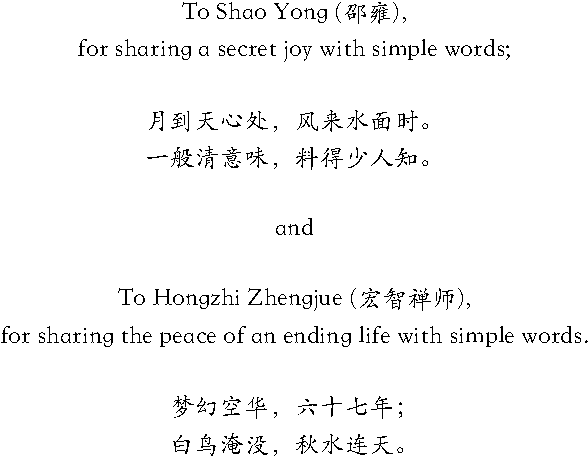
\includegraphics{images/dedication.pdf}
%	\end{center}
%
%\setlength{\abovedisplayskip}{-5pt}
%\setlength{\abovedisplayshortskip}{-5pt}

{
\hypersetup{linkcolor=}
\setcounter{tocdepth}{2}
\tableofcontents
}
\listoftables
\listoffigures
\hypertarget{preface}{%
\chapter*{Preface}\label{preface}}


The Pueblo Farming Project, or PFP, is an ongoing collaboration between
the Hopi tribe and the Crow Canyon Archaeological Center. The PFP
examines traditional Pueblo Indian farming techniques to help us
understand ancient farming in the Mesa Verde region of southwestern
Colorado. The project conducts research, develops educational programs,
and pursues Hopi interests in corn and corn farming as an essential
element of their culture. This e-book presents the methods and results
from the Pueblo Farming Project, as well as a set of lesson plans
developed for middle school students to learn about Hopi agriculture.


\includegraphics{images/by-nc-sa.png}\\
The online version of this book is licensed under the
\href{http://creativecommons.org/licenses/by-nc-sa/4.0/}{Creative
Commons Attribution-NonCommercial-ShareAlike 4.0 International License}.

\hypertarget{how-to-use-this-book}{%
\section*{How to use this book}\label{how-to-use-this-book}}


\hypertarget{saving-and-printing}{%
\section*{Saving and printing}\label{saving-and-printing}}


\hypertarget{comments-and-feedback}{%
\section*{Comments and feedback}\label{comments-and-feedback}}


\hypertarget{acknowledgments}{%
\section*{Acknowledgments}\label{acknowledgments}}


\BeginKnitrBlock{flushright}
Paul Ermigiotti, Mark Varien, Erin Bohm, and Kyle Bocinsky Cortez,
Colorado
\EndKnitrBlock{flushright}

\mainmatter

\hypertarget{introduction}{%
\chapter{Introduction}\label{introduction}}

\hypertarget{what-was-the-pfp}{%
\section{What was the PFP?}\label{what-was-the-pfp}}

\hypertarget{history}{%
\subsection*{History}\label{history}}


\hypertarget{research-goals}{%
\subsection*{Research goals}\label{research-goals}}


\hypertarget{hopi-interests}{%
\subsection*{Hopi interests}\label{hopi-interests}}


\hypertarget{educational-products}{%
\subsection*{Educational products}\label{educational-products}}


Highlight MSTFP

\hypertarget{who-were-the-participants}{%
\section{Who were the participants?}\label{who-were-the-participants}}

\hypertarget{where-did-it-take-place}{%
\section{Where did it take place?}\label{where-did-it-take-place}}

\hypertarget{when-did-it-take-place}{%
\section{When did it take place?}\label{when-did-it-take-place}}

\hypertarget{who-funded-the-pfp}{%
\section{Who funded the PFP?}\label{who-funded-the-pfp}}

\hypertarget{the-story-of-maize}{%
\chapter{The Story of Maize}\label{the-story-of-maize}}

\hypertarget{origins}{%
\section{Origins}\label{origins}}

\hypertarget{the-people-of-corn}{%
\section{The people of corn}\label{the-people-of-corn}}

\hypertarget{a-world-of-corn}{%
\section{A world of corn}\label{a-world-of-corn}}

\hypertarget{the-life-cycle-of-maize}{%
\chapter{The life-cycle of maize}\label{the-life-cycle-of-maize}}

\hypertarget{what-maize-needs-to-flourish}{%
\chapter{What maize needs to
flourish}\label{what-maize-needs-to-flourish}}

\hypertarget{soil}{%
\section{Soil}\label{soil}}

\hypertarget{water}{%
\section{Water}\label{water}}

\hypertarget{heat-and-sunlight}{%
\section{Heat and sunlight}\label{heat-and-sunlight}}

\hypertarget{gdd-sidebar}{%
\subsection*{GDD sidebar}\label{gdd-sidebar}}


\hypertarget{the-pfp-field-experiments}{%
\chapter{The PFP Field Experiments}\label{the-pfp-field-experiments}}

\hypertarget{procedure}{%
\section{Procedure}\label{procedure}}

\hypertarget{the-pfp-environment}{%
\section{The PFP environment}\label{the-pfp-environment}}

\hypertarget{soils-in-the-gardens}{%
\subsection*{Soils in the gardens}\label{soils-in-the-gardens}}


\hypertarget{cortez-weather-and-ccac-weather-stations}{%
\subsection{Cortez weather and CCAC weather
stations}\label{cortez-weather-and-ccac-weather-stations}}

\hypertarget{precipitation}{%
\subsubsection{Precipitation}\label{precipitation}}

\hypertarget{temperature}{%
\subsubsection{Temperature}\label{temperature}}

\hypertarget{gdd}{%
\subsubsection{GDD}\label{gdd}}

\hypertarget{results}{%
\section{Results}\label{results}}

\hypertarget{maize-growth-analysis}{%
\subsection*{Maize growth analysis}\label{maize-growth-analysis}}


\hypertarget{maize-production}{%
\subsection*{Maize production}\label{maize-production}}


\hypertarget{ear-diversity}{%
\subsubsection{Ear diversity}\label{ear-diversity}}

\hypertarget{yields-through-time}{%
\subsubsection{Yields through time}\label{yields-through-time}}

\hypertarget{maize-genetics}{%
\subsection*{Maize genetics}\label{maize-genetics}}


\hypertarget{what-we-learned}{%
\chapter{What we learned}\label{what-we-learned}}

\hypertarget{the-resilience-of-hopi-corn}{%
\section{The resilience of Hopi
corn}\label{the-resilience-of-hopi-corn}}

\hypertarget{improving-our-understanding-of-mesa-verde-history}{%
\section{Improving our understanding of Mesa Verde
history}\label{improving-our-understanding-of-mesa-verde-history}}

\hypertarget{culture-matters}{%
\section{Culture matters!}\label{culture-matters}}

\hypertarget{lesson-plans-for-educators}{%
\chapter{Lesson plans for educators}\label{lesson-plans-for-educators}}

\hypertarget{the-people-of-corn-1}{%
\section{The People of Corn}\label{the-people-of-corn-1}}

\hypertarget{farming-through-drought}{%
\section{Farming Through Drought}\label{farming-through-drought}}

\hypertarget{know-your-soil}{%
\section{Know Your Soil}\label{know-your-soil}}

\hypertarget{ancient-technologies}{%
\section{Ancient Technologies}\label{ancient-technologies}}

\hypertarget{the-short-blue-ear}{%
\section{The Short Blue Ear}\label{the-short-blue-ear}}

\hypertarget{references}{%
\chapter*{References}\label{references}}


\hypertarget{open-review}{%
\chapter*{Open Review}\label{open-review}}


Open Review means that you can freely read the book and easily help to
make it better. You can offer suggestions by make annotations using
\href{https://hypothes.is/}{hypothes.is}, an open source annotation
system. This is a very simple system for interacting with the book. If
you are familiar with GitHub or Git, you can also comment using
\href{https://github.com/benmarwick/bookdown-ort/issues/new}{GitHub's
issue tracker} for the book, or make a pull request. In addition to
these feedback options, this website for the book will be collecting
your implicit feedback by tracking the readership and abandonment rate
of each section of the book.

Open Review takes place before and at the same time as the book
publisher's peer review. The feedback from Open Review and peer review
will be used to create a revised manuscript. The Open Review period will
end when the final manuscript is submitted to the publisher.

The concept of Open Review, as it is implemented here, is taken from
\href{https://twitter.com/msalganik}{Matthew Salganik's}
\href{http://www.openreviewtoolkit.org/}{Open Review Toolkit}. Much of
the text on this page comes from the
\href{http://www.bitbybitbook.com/en/open-review/}{Open Review Toolkit
About page} and the \href{http://www.bitbybitbook.com/en/privacy/}{Open
Review Toolkit Privacy and Consent page}

\hypertarget{faq-about-open-review}{%
\section*{FAQ about open review}\label{faq-about-open-review}}


\hypertarget{what-kind-of-feedback-are-you-looking-for}{%
\subsection*{What kind of feedback are you looking
for?}\label{what-kind-of-feedback-are-you-looking-for}}
\addcontentsline{toc}{subsection}{What kind of feedback are you looking
for?}

Open Review is not just about catching typos. Rather, Open Review is
designed to collect all types of feedback, and I'd particularly welcome
any feedback that you have about the substance of the book. Are there
sections that you find particularly confusing? Are their points that you
find particularly important? Am I making claims that you think need to
be refined? Are there parts of the book that you think should be
removed? When in doubt, I think you should follow one of the main
principles at Wikipedia:
\href{https://en.wikipedia.org/wiki/Wikipedia:Be_bold}{Be bold}.

\hypertarget{can-i-see-the-annotations-that-others-are-making}{%
\subsection*{Can I see the annotations that others are
making?}\label{can-i-see-the-annotations-that-others-are-making}}
\addcontentsline{toc}{subsection}{Can I see the annotations that others
are making?}

Yes, all the annotations are public. You can see them on right hand side
of the each page or you can read them in
\href{https://hypothes.is/stream?q=benmarwick-bookdown-ort}{stream
form}.

\hypertarget{what-are-the-benefits-for-readers}{%
\subsection*{What are the benefits for
readers?}\label{what-are-the-benefits-for-readers}}


You get to read the manuscript and help make it better.

\hypertarget{what-are-the-benefits-for-authors-and-publishers}{%
\subsection*{What are the benefits for authors and
publishers?}\label{what-are-the-benefits-for-authors-and-publishers}}
\addcontentsline{toc}{subsection}{What are the benefits for authors and
publishers?}

The Open Review process will benefit both authors and publishers, even
if they have no interest in increasing access to knowledge. The process
will lead to higher manuscript quality through the explicit and implicit
feedback. Further, the Open Review process will provide valuable data
that can be used during that marketing of the book.

\hypertarget{has-anyone-ever-done-something-like-this-before}{%
\subsection*{Has anyone ever done something like this
before?}\label{has-anyone-ever-done-something-like-this-before}}
\addcontentsline{toc}{subsection}{Has anyone ever done something like
this before?}

This is based on \href{https://twitter.com/msalganik}{Matthew
Salganik's} \href{http://www.openreviewtoolkit.org/}{Open Review
Toolkit}. He's written about some related efforts here:
\url{http://www.bitbybitbook.com/en/open-review/}

\hypertarget{what-kind-of-information-are-you-collecting-and-how-will-that-information-be-used}{%
\subsection*{What kind of information are you collecting and how will
that information be
used?}\label{what-kind-of-information-are-you-collecting-and-how-will-that-information-be-used}}
\addcontentsline{toc}{subsection}{What kind of information are you
collecting and how will that information be used?}

Please read our privacy and consent policy, below.

\hypertarget{how-i-can-learn-more-about-traditional-peer-review-of-academic-books}{%
\subsection*{How I can learn more about traditional peer review of
academic
books?}\label{how-i-can-learn-more-about-traditional-peer-review-of-academic-books}}
\addcontentsline{toc}{subsection}{How I can learn more about traditional
peer review of academic books?}

The AAUP recently published
\href{http://www.aaupnet.org/resources/for-members/handbooks-and-toolkits/peer-review-best-practices}{a
report} on best practices for peer review.

\hypertarget{can-i-do-this-with-my-book}{%
\subsection*{Can I do this with my
book?}\label{can-i-do-this-with-my-book}}


Sure. Check out the code for this website at
\url{https://github.com/benmarwick/bookdown-ort/} for more about how we
did it.

\hypertarget{i-have-a-different-question-about-open-review.-how-can-i-get-in-touch}{%
\subsection*{I have a different question about Open Review. How can I
get in
touch?}\label{i-have-a-different-question-about-open-review.-how-can-i-get-in-touch}}
\addcontentsline{toc}{subsection}{I have a different question about Open
Review. How can I get in touch?}

Send an email to \texttt{bmarwick@uw.edu}

\hypertarget{privacy-and-consent-policy}{%
\section*{Privacy and Consent Policy}\label{privacy-and-consent-policy}}


\hypertarget{overview}{%
\subsection*{Overview}\label{overview}}


On this website, we are making the complete text of the book available
at no cost. While you are reading the book, we are measuring reader
behavior in aggregate. For example, we are measuring which sections of
the book get read most often. This data will help us improve the book.
Everything we are doing is common on modern websites. We describe it in
more detail below.

\hypertarget{what-information-do-we-collect}{%
\subsection*{What information do we
collect?}\label{what-information-do-we-collect}}


We use \href{https://analytics.google.com/}{Google Analytics} to collect
information about how you interact with this website. Further, like most
websites, we use
\href{https://en.wikipedia.org/wiki/HTTP_cookie}{cookies} to enhance
your experience, gather general visitor information, and track visits to
our website. Please refer to the ``do we use cookies?'' section below
for information about cookies and how we use them.

\hypertarget{how-do-we-use-your-information}{%
\subsection*{How do we use your
information?}\label{how-do-we-use-your-information}}


Any of the information that we collect may be used for research, to
improve the book, and to help sell the book.

\hypertarget{how-do-we-protect-your-information}{%
\subsection*{How do we protect your
information?}\label{how-do-we-protect-your-information}}


We implement a variety of security measures to maintain the safety of
the information that you provide us.

Most of the browsing information that we have is stored Google
Analytics, and you can read more about their
\href{https://support.google.com/analytics/answer/6004245?hl=en}{security
and privacy principles}.

Annotations that you add are managed by
\href{https://hypothes.is/}{hypothes.is}, and you can read more about
their \href{https://hypothes.is/terms-of-service/}{terms of service}.

Our website is hosted by \href{https://pages.github.com/}{Github Pages},
and you can read more about Github's
\href{https://help.github.com/articles/github-terms-of-service/}{terms
of service}.

\hypertarget{do-we-use-cookies}{%
\subsection*{Do we use cookies?}\label{do-we-use-cookies}}


Yes. Cookies are small files that a site or its service provider
transfers to your computer's hard drive through your web browser (if you
allow) that enables the sites or service providers systems to recognize
your browser and capture and remember certain information.

In order to offer you a better site experience, we use cookies to
understand and save your preferences for future visits and to compile
aggregate data about site traffic.

\hypertarget{do-we-disclose-any-information-to-outside-parties}{%
\subsection*{Do we disclose any information to outside
parties?}\label{do-we-disclose-any-information-to-outside-parties}}
\addcontentsline{toc}{subsection}{Do we disclose any information to
outside parties?}

We do not sell, trade, or otherwise transfer to outside parties your
personally identifiable information except trusted third parties who
assist us in operating our website, conducting research, or providing a
service to you, so long as those parties agree to keep this information
confidential. We may also release your information when we believe
release is appropriate to comply with the law, enforce our site
policies, or protect ours or others' rights, property, or safety.

\hypertarget{third-party-links}{%
\subsection*{Third party links}\label{third-party-links}}


Occasionally, at our discretion, we may include links to third party
websites. These third party sites have separate and independent privacy
policies. We, therefore, have no responsibility or liability for the
content and activities of these linked sites. Nonetheless, we seek to
protect the integrity of our site and welcome any feedback about these
sites.

\hypertarget{website-hosting}{%
\subsection*{Website hosting}\label{website-hosting}}


Our website is hosted by Github Pages, and you can read more about
Github's terms of service.

\hypertarget{your-consent}{%
\subsection*{Your consent}\label{your-consent}}


By using our site, you consent to our privacy policy.

\hypertarget{questions}{%
\subsection*{Questions}\label{questions}}


If you have any questions, please send us an email
\texttt{kbocinsky@crowcanyon.org}

\hypertarget{changes-to-our-privacy-and-consent-policy}{%
\subsection*{Changes to our Privacy and Consent
Policy}\label{changes-to-our-privacy-and-consent-policy}}
\addcontentsline{toc}{subsection}{Changes to our Privacy and Consent
Policy}

We reserve the right to change our privacy policy from time to time at
our sole discretion. Please periodically check this section to review
the current version of the Privacy and Consent Policy. All our previous
policies are presented below, and we will continue to update this page
if any changes are needed.

\bibliography{book.bib,packages.bib}

\backmatter
\printindex

\end{document}
